\documentclass[mathserif]{beamer}
\usepackage{mathtools}
\usepackage{amssymb}
\usepackage{bm}
\usepackage{graphicx}
\usetheme{Copenhagen}

\begin{document}
	\title[Analyzing Stochastic Time-Series Data]{Techniques for Analyzing Stochastic Time-Series Data}
	\author[Castleberry \and Oubre \and Yu]{Dennis Castleberry \and Brandon Oubre \and Haikou Yu}
	\date{\today}
	\frame{\titlepage}
	
	\section{Naive Bayes}
	\subsection{Overview}
	\begin{frame}
		\frametitle{The Naive Bayes Classifier}
		\begin{itemize}
			\item Reduce classification to probability. What is \(P(class | attribute1, attribute2, ..., attributeN)\).
			\item Assumes that each attribute is independent of the others. (Hence the ``Naive'' nickname.)
			\item For example, let's consider if a car is stolen using \(P(stolen | Color, Type)\). Naive Bayes will assume \(color=red\) and \(type=sportscar\) to be independent.
			\item Naive Bayes is not sensitive to irrelevant attributes, since the probabilities of such attributes will be similar for all classes.
			\item Naive Bayes is quick to train, as it requires only one pass-though of the training data.
		\end{itemize}
	\end{frame}
	
	\subsection{Example}
	\begin{frame}
		\frametitle{Naive Bayes in Action}
		\begin{center} 
			\textbf{Training Data} \\
			\begin{tabular}{c | c | c || c}
				\textbf{Over 170cm} & \textbf{Eye Color} & \textbf{Hair Length} & \(\boxed{\textbf{Sex}}\) \\ \hline \hline
				No & Blue & Short & Male \\ \hline
				Yes & Brown & Long & Female \\ \hline
				No & Blue & Long & Female \\ \hline
				Yes & Brown & Short & Male \\ \hline
				Yes & Brown & Short & Female \\
			\end{tabular}  \\
			\small{Only discrete values shown, but we can still interpret real data using normal distributions!}
		\end{center}
			Suppose we are given an unseen data point \(\langle No, Blue, Short \rangle\). What should we classify it as?
	\end{frame}
	
	\begin{frame}
		\frametitle{Naive Bayes in Action}
		\begin{tabular}{l}
		\(P(Male|No,Blue,Short)\) \\
		\(=\dfrac{P(No,Blue,Short|Male) P(Male)}{P(No,Blue,Short)}\) \\
		\(= \alpha P(Male)\bm{P(No|Male)P(Blue|Male)P(Short|Male)}\) \\
		\(=\alpha \times \frac{2}{5} \times \frac{1}{2} \times \frac{1}{2} \times \frac{2}{2} = \boxed{0.1\alpha}\) \\ \\
		\hline \\
		\(P(Female|No,Blue,Short)\) \\
		\(=\alpha P(Female)P(No|Female)P(Blue|Female)P(Short|Female)\) \\
		\(= \alpha \times \frac{3}{5} \times \frac{1}{3} \times \frac{1}{3} \times \frac{1}{3} = \boxed{0.0\overline{2}\alpha}\) \\
		\end{tabular} \\
		\vspace{10px}
		Since \(P(Male|Data) > P(Female|Data)\), we classify the unseen point as Male. For multiple classes, just select the class with the greatest probability!
	\end{frame} 
	
	\section{Support Vector Machine}
	\subsection{Overview}
	\begin{frame}
		\frametitle{Support Vector Machines (SVM)}
		\begin{itemize}
			\item Idea is to draw a line (or hyperplane) between the data points of different classes. Classify unseen data by testing which side of the line it is on.
			\item Focus on support vectors, or the points that would change the line if removed from the training data.
			\item Find an optimal line to separate the data. Such a line will have the larger margin for data points and should mis-classify the least number of new points.
			\item If data is not linearly separable, then a transformation of the data to a new basis can be performed. The data may be linearly separable in the new basis.
		\end{itemize}
	\end{frame}
	
	\subsection{Example}
	\begin{frame}
		\frametitle{SVM Example}
		\begin{columns}[t]
			\column{.5\textwidth}
			\begin{figure}
				\centering
				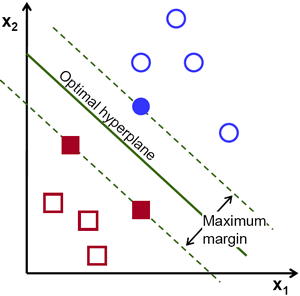
\includegraphics[keepaspectratio,scale=2]{SVM.png} \\ \vspace{5px}
				\Tiny{Image from \url{http://docs.opencv.org/doc/tutorials/ml/introduction_to_svm/introduction_to_svm.html}}
			\end{figure}
			
			\column{.5\textwidth}
			\begin{itemize}
				\item Solid Figures are support vectors.
				\item Due to the maximized margin, unseen figures can be closer to the line than the support vectors and still be correctly classified.
				\item It is easy to see how new points are classified.
			\end{itemize}
		\end{columns}
	\end{frame}
	
	\section{Neural Network}
	\subsection{Overview}
	\begin{frame}
		\frametitle{Neural Networks}
		\begin{itemize}
			\item Inspired by biological neurons.
			\item Neurons maintain a weighted sum of their inputs. The result of this sum is passed into a function and output. (A step function produces on/off signals while a Sigmoid will produce continues levels of activation.)
			\item The network can be trained by adjusting the weights of the inputs to each neuron.
			\item In a feed-forward network, the backwards propagation algorithm accomplishes this.
			\item Networks with multiple layers can classify various types of non-linearly separable data.
		\end{itemize}
	\end{frame}
	
	\subsection{Structure and Classification}
	\begin{frame}
		\frametitle{An Artificial Neuron}
		\begin{figure}
			\centering
			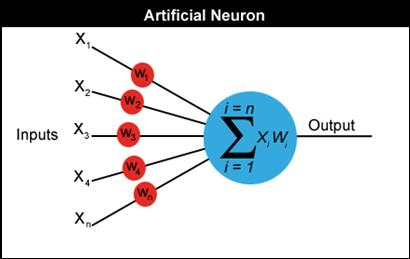
\includegraphics[keepaspectratio,scale=.95]{NN_1.jpg} \\
			\Tiny{Image from \url{http://www.ai-junkie.com/ann/evolved/nnt1.html}}
		\end{figure}
	\end{frame}
	
	\begin{frame}
		\frametitle{Neural Network Classification}
		\begin{columns}[t]
			\column{.5\textwidth}
			\begin{figure}
				\centering
				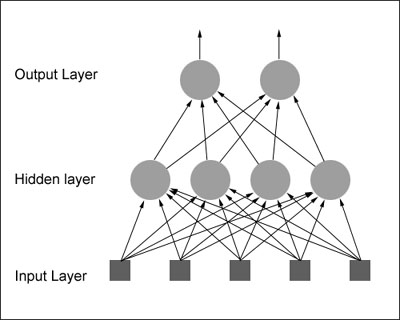
\includegraphics[keepaspectratio,scale=0.4]{NN_2.jpg} \\ \vspace{5px}
				\Tiny{Image from \url{http://www.ai-junkie.com/ann/evolved/nnt1.html}}
			\end{figure}
			
			\column{.5\textwidth}
			\begin{itemize}
				\item Information is fed into the input layer.
				\item The outputs of the neurons in the output layer represent classifications.
				\item Hidden layers perform intermediary manipulations of signals. More hidden layers can be added as needed.
			\end{itemize}
		\end{columns}
	\end{frame}
	
\end{document}